% %%%%%%%%%%%%%%%%%%%%%%%%%%%%%%%%%%%%%%%%%%%%%%%%%%%%%%%%%%%%%%%%%%%%%
% %% Theory %%
% Introduction
% %%%%%%%%%%%%%%%%%%%%%%%%%%%%%%%%%%%%%%%%%%%%%%%%%%%%%%%%%%%%%%%%%%%%%

\section{Introduction}
\label{sec:theory:intro}

TODO


%background
In Figure~\ref{fig:banded_mat_def}, we illustrate a banded, square matrix of dimension $M$.
We define $w_B$ as the width of the banded region, or \textit{bandwidth}, as shown in \textit{red} in the figure. 
Sometimes it is easier to refer to the half-\textit{bandwidth}, $w_{hB}$, which respects the relation $w_B = 2w_\mathit{hB} - 1$.
The average density in the band and out of the band is defined as $d_\mathit{IB}$ and $d_\mathit{OB}$, respectively.
In a \textit{perfectly banded} matrix, there are no elements outside the band, thus $d_\mathit{OB} = 0$.

\begin{figure}[htbp]
    \centering
    % \begin{minipage}[b]{0.33980583\linewidth} % 17.5/51.5
    %     \begin{figure}[H]
    %         \centering
    %         
\includegraphics[width=\linewidth]{Chapter_Theory/Figures/PDF/MatrixDef.pdf}
    %         \caption{Banded Matrix Definition}
    %         \label{fig:banded_mat_def}
    %     \end{figure} 
    % \end{minipage}
    % \hfill
    \begin{minipage}[b]{0.63106796\linewidth} % 32.5/51.5
        \begin{figure}[H]
            \centering
            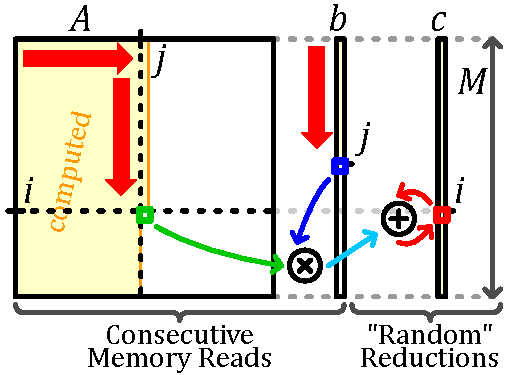
\includegraphics[width=\linewidth]{Chapter_Theory/Figures/PDF/MatrixSpMVRep.pdf}
            \caption{Visual Representation of \algo{OP} SpMV Computation}
            \label{fig:op_spmv_rep}
        \end{figure}
    \end{minipage}
\end{figure}

Sparse matrices are used in many kernels, such as sparse matrix-vector (SpMV) and sparse matrix-matrix multiplication (SpMM).
These kernels can be implemented with several algorithms.
Many works~\cite{Isaac2024_SoA, Mukkara2019_PHI, Pal2018_OuterSPACE} have shown that the \textit{Outer-Product} (\algo{OP}) algorithm has the potential to enhance performance, if computed with an adapted hardware architecture.
For sparse kernels, the performance is almost always limited by the indirect accesses induced by the sparse formats.
The indirections are ``random'' and have limited spatial and temporal locality, limiting the effectiveness of traditional caches.
For \algo{OP} algorithms, these indirect accesses occur when updating the output vector, which are referred to as ``scatter updates''.

Many software solutions focus on improving performance, using conventional compute hardware including CPUs and GPUs~\cite{MOHAMMED_2022_SPARSE}, but since the performance limitation comes from the memory system, custom hardware solutions are required.
PHI~\cite{Mukkara2019_PHI}, SortCache~\cite{Srikanth2021_SortCache} and ASA~\cite{Zhang2022_ASA} modify the cache hierarchy for an existing processor to support scatter updates.
This type of accelerator, called a \textit{reduction cache}, has the advantage of being general purpose, offering a performance improvement to any algorithm requiring ``random'' scatter updates.
The focus of this paper is a new \textit{reduction cache} architecture, which exploits the coarse- and fine-grained structure of the matrix, to improve performance, unlike previous solutions.

Our analysis is focussed on the \algo{OP} SpMV kernel, \mbox{$A \times b = c$}, shown in Algorithm~\ref{alg:op_spmv}.
The solution is equally applicable to SpMM kernels with \textit{Gustavson}'s algorithm~\cite{Gustavson1978_GustAlgo} or other ``push''-type graph algorithms.
\algo{OP} SpMV is the sparse version of matrix-vector multiplication that simply consists in $c_{i} \acc A_{i,j} \times b_j$ for all $0 \leqslant i, j \leqslant M-1 \in \mathbb{N}$, computed column-first.
It behaves differently than the row-first, \textit{Inner-Product} version.
The matrix $A$ is sparse and is usually stored in the CSC sparse format (\textit{Compressed Sparse Column})~\cite{Saad2003_CSR}, which consists in three 1D-tables: $\mathit{val}$ of size $nnz$, containing all the non-zero elements, sorted by column; $\mathit{idx}$ of size $nnz$, containing the row-index of every non-zero element; $\mathit{ptr}$ of size $M+1$, containing the position of each column in tables $\mathit{val}$ and $\mathit{idx}$.
The vectors $b$ and $c$ are dense (one table each).

% \begin{algorithm}[htbp]
%     \caption{\algo{OP} SpMV: $A \times b = c$}\label{alg:op_spmv}
%     \For(\Comment*[f]{Column-first}){$j \in \ldb0, M-1\rdb$}{
%         \For{$\mathit{pos} \in \ldb\mathit{ptr}_j, \mathit{ptr}_{j+1}-1\rdb$}{
%             $\mathit{i} \gets \mathit{idx}_{\mathit{pos}}$\;
%             $c_{\mathit{i}} \gets c_{\mathit{i}} + \mathit{val}_{\mathit{pos}} \times b_j$\Comment*[r]{RED}
%         }
%     }
% \end{algorithm}

When computing an \algo{OP} SpMV, the matrix is read column by column, left to right, traversing the columns top to bottom, shown in Figure~\ref{fig:op_spmv_rep}.
Each non-zero element of row $i$ (horizontally) will eventually be accumulated into the output vector $c$ at index $i$.
In our representation, we show the output vector $c$ at the right of the matrix.
Since the traversal of the matrix $A$ is column-wise, each element of $c$ is progressively updated.

With the \algo{OP} algorithm and CSC format, reads to $A$ and $b$ occur on consecutive addresses, both being read once.
Caches benefit from the spatial locality of these accesses and effectively mask the external memory latency.
Because $A$ is sparse, the reads and writes to $c$ do not necessarily occur on consecutive addresses.
This is due to indirections when accessing $c$ via the $\mathit{idx}$ table of $A$: $c_{idx_{pos}}$.
The obstacle to high performance are these ``random'' scatter updates to $c$ and in the next sections, we study the cache behavior when updating $c$.

In \algo{OP} SpMV, the accesses that occur to $c$ consist of a read of $c_i$, a modification (accumulation with partial product $\mathit{val}_\mathit{pos} \times b_j$) and a write to update $c_i$, which is referred to as a \textit{reduction} (line 4 of Algorithm~\ref{alg:op_spmv}).
For other ``push''-type algorithms, the modify operation may change (e.g. logical OR...) but the read-modify-write pattern is the same.
\textit{Reduction caches} are specialized data-caches that can natively perform \textit{reductions}.
Indeed, instead of considering the \textit{reduction} as two separate memory transactions, it becomes a single memory transaction, $\mathit{RED}(\mathit{address}, \mathit{value})$.
This new operation can be implemented as a single, ``fire-and-forget'' instruction, meaning the processor does not need to wait for a response, unlike a load instruction.
The value of the \textit{reduction} is then simply stored or accumulated in the cache, and merged to main memory when the cache-line must be evicted.
This ``write-back''-like policy removes unnecessary memory traffic and masks memory read response latency.
The \textit{reduction cache} computes accumulations internally, using a local arithmetical unit, a form of near-memory computing.
Existing accelerators such as PHI, SortCache and ASA are based on a \textit{reduction cache}.
In addition, they each have their own unique approach to manage the spatial irregularity of the \textit{reductions}.
Indeed, a simple \textit{reduction cache} is not sufficient to manage these ``random'' accesses, as we will show in Section~\ref{sec:theory}.

In our analysis of \textit{reduction caches}, we use a set-associative configuration, with $8$ byte elements which we consider as the basic memory unit.
$s_C$ is the size of the cache, in elements.
The cache is divided into \textit{sets}, ways and cache-lines, of size $S$, $W$ and $l$, respectively.
Thus, $s_C = S \times W \times l$ elements.

Our focus is on banded matrices, thus for each non-zero element, we must determine if it is in or out of the band.
This could be done in the inner-loop of the algorithm (lines 4-7 of Algorithm~\ref{alg:op_spmv}), by checking $|j - pos| \leqslant w_\mathit{hB}$, but this adds many instructions in the critical inner-loop.
To avoid this overhead, we propose a dedicated sparse format called BaCSC (\textit{Banded CSC}) that adds the in- or out-of-band information in the $\mathit{ptr}$ table.
In the standard CSC $\mathit{ptr}$ table, two consecutive entries of indices $k$ and $k+1$ indicate the position in the $\mathit{idx}$ and $\mathit{val}$ tables of the first non-zero element of column $k$ and $k+1$.
In the BaCSC $\mathit{ptr}$ table, we add two entries, to indicate the position in the $\mathit{idx}$ and $\mathit{val}$ tables of the first and the last non-zero element of the in-band region of column $k$.
This extended $\mathit{ptr}$ table has a size of $3M+1$, but enables the location of the band to be determined in the outer-loop, reducing the instructions in the inner-loop.

\clearpage